\chapter{Experimentos}
\label{experimentos}

Os operadores propostos nesta pesquisa podem ser compostos de diferentes formas, 
construindo diversas heurísticas que podem encontrar soluções distintas para 
\ac{tmap}. Assim, este capítulo tem dois objetivos. O primeiro é encontrar as 
melhores combinações de operadores. O segundo é comparar as heurísticas que 
obtiveram melhores resultados com abordagens propostas por outros autores.

Os operadores descritos neste trabalho foram implementados na linguagem de 
programação Java\footnote{\url{http://java.com/pt_BR/}}. A principal razão para 
a adoção desta linguagem foi o \textit{Simple Patrol}, simulador da \ac{tmap}, 
desenvolvido pelo grupo de pesquisa sobre Patrulha Multiagente da Universidade 
Federal Rural de Pernambuco, utilizado para realizar os experimentos desta 
pesquisa. Os operadores foram desenvolvidos de forma compatível com a biblioteca 
jMetal\footnote{\url{http://jmetal.sourceforge.net/}} \citep{Durillo2011}, que 
disponibiliza diversos algoritmos evolucionários facilmente adaptáveis para 
qualquer problema que possa ser modelado em classes Java.

Uma vez que os operadores estavam implementados e importados no simulador da 
\ac{tmap}, foram realizados diversos experimentos divididos em dois grupos. O 
primeiro com o objetivo de encontrar as melhores abordagens evolucionárias para 
\ac{tmap} e o segundo com a finalidade de comparar estas abordagens com as 
publicadas por outros autores.

A Métrica utilizada para avaliar os indivíduos se manteve constante em todos 
os experimentos. Foi selecionada a média quadrática dos intervalos, pois segundo 
\citep{sampaiophd} ela reflete o equilíbrio entre as métricas de intervalo 
médio, intervalo máximo e desvio padrão dos intervalos e, por isso, é uma boa 
métrica para a \ac{tmap}.

Abaixo, estão listados alguns parâmetros que, embora não influenciem diretamente 
nos algoritmos evolucionários, tem grande impacto nas respostas obtidas.

\begin{itemize}
	% Número Máximo de Avaliações
	\item Todos os algoritmos evolucionários descritos no \chapref{alg_evo}, 
	executam seu \textit{loop} principal até "não haja mais tempo". Esse tempo é 
	representado pelo parâmetro \textbf{número máximo de avaliações}. Toda vez 
	que o algoritmo evolucionário avalia a aptidão de um indivíduo, ele 
	incrementa o contador do número de avaliações. Quando esse contador chegar 
	no número máximo de avaliações, o algoritmo evolucionário para.
	% Número de turnos a cada avaliação
	\item Cada vez que uma avaliação de aptidão de um indivíduo é requisitada, 
	uma instância do \textit{Simple Patrol} é iniciada. Essa instância simula 
	a solução correspondente ao indivíduo e retorna o valor da métrica, que é 
	utilizado como aptidão. A solução é simulada por um número pré-definido de 
	unidades de tempo, que corresponde ao parâmetro \textbf{número de turnos}.
	% Número de agentes
	\item A \textbf{quantidade de agentes} é outro número que influi no 
	desempenho das soluções para a \ac{tmap}. A medida que este número cresce, 
	fica cada vez mais simples patrulhar uma mesma quantidade de pontos de 
	interesse com alta frequência. \citep{sampaiophd} descobriu 
	experimentalmente que não vale a pena manter a relação entre a quantidade de 
	agentes e a quantidade de nós acima de um terço, pois, a partir desse número, 
	estratégias bem distintas passam a ter desempenhos muito próximos.
\end{itemize}

Outro ponto importante são os mapas que foram utilizados nos experimentos. Esta 
pesquisa se valeu de três grafos diferentes para testar e comparar os algoritmos 
evolucionários. Eles estão ilustrados na \figref{fig:mapas}.

\begin{figure}[tp]
	\caption[Mapas utilizados nos experimentos]{Mapas utilizados nos 
		experimentos}
	\centering
	\begin{minipage}{0.5\textwidth}
		\centering
		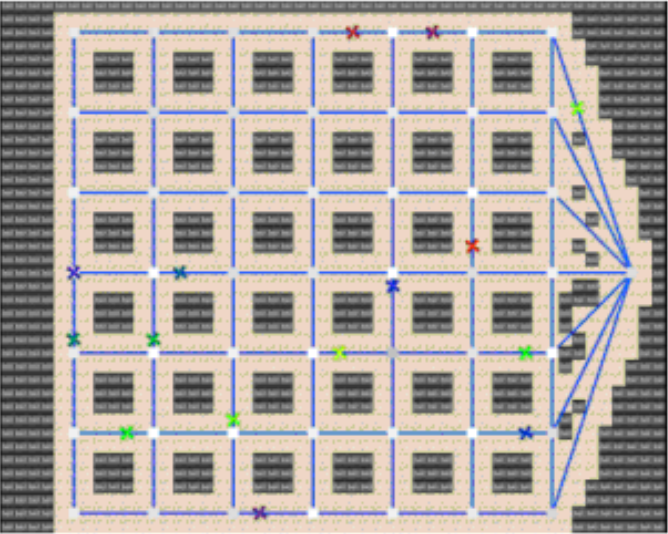
\includegraphics[width=0.9\linewidth]{images/mapa_grid.png}
		\label{fig:grid}
		\captionof*{figure}{Mapa \textit{grid}}
	\end{minipage}\hfill
	\begin{minipage}{0.5\textwidth}
		\centering
		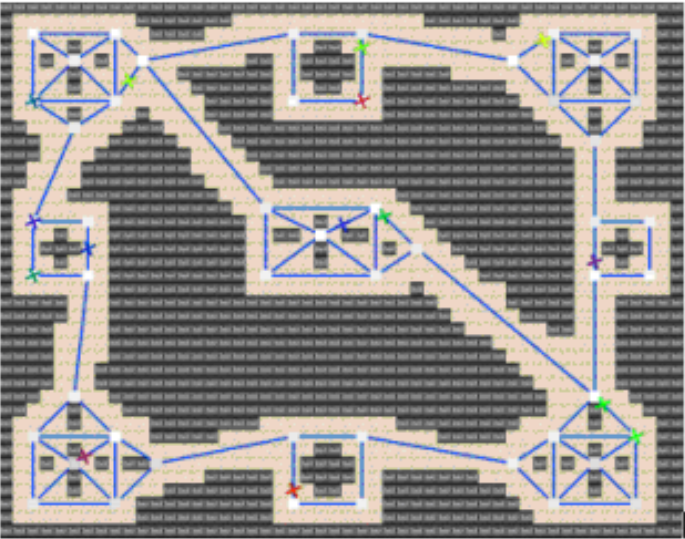
\includegraphics[width=0.9\linewidth]{images/mapa_ilhas.png}
		\label{fig:islands}
		\captionof*{figure}{Mapa \textit{islands}}
	\end{minipage}
	\begin{minipage}{0.5\textwidth}
		\centering
		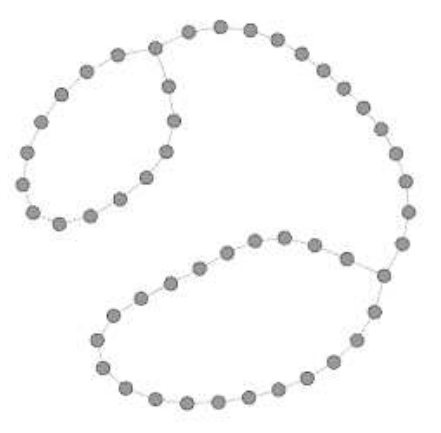
\includegraphics[width=\linewidth]{images/mapa_cicles_corridor.png}
		\label{fig:cicles_corridor}
		\captionof*{figure}{Mapa \textit{cicles corridor}}
	\end{minipage}
	\caption*{Fonte: \citep{sampaiophd}}
	\label{fig:mapas}
\end{figure}

Nas seções seguintes, serão discutidos os dois grupos de experimentos 
realizados. Eles foram chamados de Experimentos de \textit{Tuning} e de 
comparação.

\section{Experimentos de \textit{Tuning}}

\textit{Tuning} pode ser traduzido, do inglês, para ajuste. Esta seção tem como 
finalidade descrever e apresentar os resultados dos experimentos desenvolvidos 
para buscar o ajuste dos operadores que compõem as melhores heurísticas 
evolucionárias estudadas nesta pesquisa. Por exemplo, qual seria a melhor forma 
de inicializar um indivíduo? Existem ao todo doze formas diferentes de compor 
o operador de inicialização de indivíduos de uma heurística evolucionária 
utilizando os operadores propostos no \chapref{chp:abordagens}.

Primeiramente, foram realizados experimentos para determinar um número máximo 
de avaliações que permitisse distinguir os desempenhos das heurísticas nos 
demais experimentos. Enquanto o número máximo de avaliações variou entre 10 mil 
e 150 mil, os demais parâmetros permaneceram fixados:

\begin{itemize}
	\item Algoritmo utilizado: Estratégia Evolucionária $(\mu + \lambda)$
	\item Número de turnos: 2 mil
	\item Número de agentes: 5
	\item $\mu$: 30
	\item $\lambda$: 180
	\item Mapa: \textit{islands}
	\item Criação de indivíduos: \textit{Random Centering}, 
	\textit{Random Partitioning}, \textit{Random Path Building}
	\item Mutação: \textit{Half Add Half Sub Small Changes}
\end{itemize}

O resultado apontava que 30 mil avaliações eram suficientes para as 
estratégias evoluírem de soluções notadamente ruins para soluções ao ponto 
de convergir.

Depois, foram testados os tamanhos de população. Nos algoritmos genéticos, 
esse parâmetro diz respeito à quantidade de indivíduos a cada geração. 
Já nas estratégias evolucionárias existem dois parâmetros relacionados ao tamanho 
da população: $\mu$ e $\lambda$, como foi discorrido no \chapref{alg_evo}. Um 
experimento similar ao anterior foi realizado: as diferenças eram o número de 
avaliações agora fixado em 30 mil, mas com $\mu$ e $\lambda$ variando para as 
Estratégias Evolucionárias e o tamanho da população variando para o algoritmos 
genéticos. Todos os quatro algoritmos apresentados nesse trabalho foram testados 
individualmente. $\lambda$ e o tamanho da população variaram entre 72 e 180. 
$\mu$ variou entre $1/4$, $1/5$ e $1/6$ do valor de $\lambda$.

Os resultados obtido foram:
\begin{itemize}
	\item População de 96 indivíduos para o Algoritmo Genético
	\item População de 110 indivíduos para o Algoritmo Genético de Estado Estável
	\item $\mu = 18$ e $\lambda = 90$ para a Estratégia Evolucionária 
	$(\mu + \lambda)$
	\item $\mu = 26$ e $\lambda = 156$ para a Estratégia Evolucionária 
	$(\mu, \lambda)$
\end{itemize}

